\section{Motivation}
\label{sec:motivation}

\subsection{Fine-Grained EKF Execution Is Latency-Bound}
\label{subsec:motivation-latency}

The CPU fp64 implementation processes approximately 1,866 filter steps per second and serves as the numerical reference; its representative characteristics are summarized in \Cref{tab:baseline-characteristics}. Moving the same tensor-level computation directly to the GPU does not produce a corresponding speedup. Each EKF step contains a dependent chain of tensor construction, element-wise arithmetic, trigonometric functions, and small matrix operations. The eager implementation expands this modest amount of arithmetic into roughly 531 CUDA kernel launches per step. As a result, dispatch, synchronization, and recurrent-state transfers occupy a substantial part of the execution time.

Device measurements confirm that the baseline is latency-bound. A single trajectory activates only a small portion of the GPU, and its measured SM throughput is approximately $0.27\%$. The launch cost of a general-purpose small-matrix kernel can approach or exceed the cost of its arithmetic. CUDA Graph replay reduces repeated host dispatch, but the captured graph still executes the fine-grained dependent kernels and transfers state between them. These observations motivate a larger execution scope that can preserve recurrent data across filter steps and eliminate fragmented device execution.

\begin{table}[H]
  \centering
  \caption{Representative characteristics of the baseline positioning workload (GPU utilization measured on an H20).}
  \label{tab:baseline-characteristics}
  \begin{tabular}{@{}lr@{}}
    \toprule
    Characteristic & Value \\
    \midrule
    Trajectory length & 166,667 steps \\
    EKF state dimension & 15 \\
    Maximum logical matrix size & $15\times15$ \\
    Naive kernels per step & approximately 531 \\
    CPU fp64 throughput & 1,866 steps/s \\
    Naive GPU SM throughput & approximately 0.27\% \\
    \bottomrule
  \end{tabular}
\end{table}

\subsection{Precision Choices Have Unequal Numerical and Hardware Effects}
\label{subsec:motivation-precision}

Uniformly changing the precision of the estimator overlooks the different roles of its components. Sensor samples are noisy external inputs that are consumed once, whereas position, velocity, attitude, error state, and covariance are carried through the complete trajectory. Rounding in these recurrent quantities can accumulate through repeated propagation and feedback. Accuracy measured for an isolated filter step is therefore insufficient to determine whether a reduced-precision configuration is acceptable over a long simulation.

Lower nominal precision also does not guarantee lower execution time. TensorFloat-32 and Tensor Core paths may require conversion, padding, and scheduling work that is difficult to amortize for the small matrices in this estimator. Storage precision, recurrent arithmetic, and matrix-multiplication mode consequently present different accuracy and performance trade-offs. This behavior motivates component-level precision choices evaluated with both hardware measurements and complete-trajectory numerical error. \Cref{fig:precision-tradeoff} combines the two views for the complete trajectory: throughput (bars) and the per-axis deviation from the all-fp32 reference (lines) share one panel, so accuracy and performance can be read together for each configuration.

We additionally isolate one precision decision at a time over the complete 166,667-step trajectory, while retaining fp32/IEEE arithmetic for all remaining components. As summarized in \Cref{tab:precision-isolation}, fp16 sensor input causes only limited additional error, whereas bfloat16 input substantially amplifies the vertical error. TF32 matrix products introduce a measurable X-axis deviation, and storing the recurrent navigation state in fp16 causes the long-horizon filter to diverge. These outcomes distinguish once-consumed sensor data from values repeatedly propagated through the recursion and motivate the component-aware scheme in \Cref{sec:methodology}.

\begin{table}[H]
  \centering
  \caption{Component-isolation precision study over the full 166,667-step trajectory in the fused scan (\Cref{subsec:kernel-fusion}), measured on an H20. Each row lowers one component while the remaining components use fp32/IEEE arithmetic; values report the per-axis RMSE difference (mm) against the all-fp32 reference.}
  \label{tab:precision-isolation}
  \begin{tabular}{@{}llrr@{}}
    \toprule
    Component & Lowered mode & $\Delta$X (mm) & $\Delta$Z (mm) \\
    \midrule
    Sensor input & fp16 & $0.11$ & $2.19$ \\
    Matrix products & TF32 & $4.82$ & $0.31$ \\
    Sensor input & bfloat16 & $11.01$ & $1005.84$ \\
    Recurrent state & fp16 storage & $280753.72$ & $-0.30$ \\
    \bottomrule
  \end{tabular}
\end{table}

\begin{figure}[!t]
  \centering
  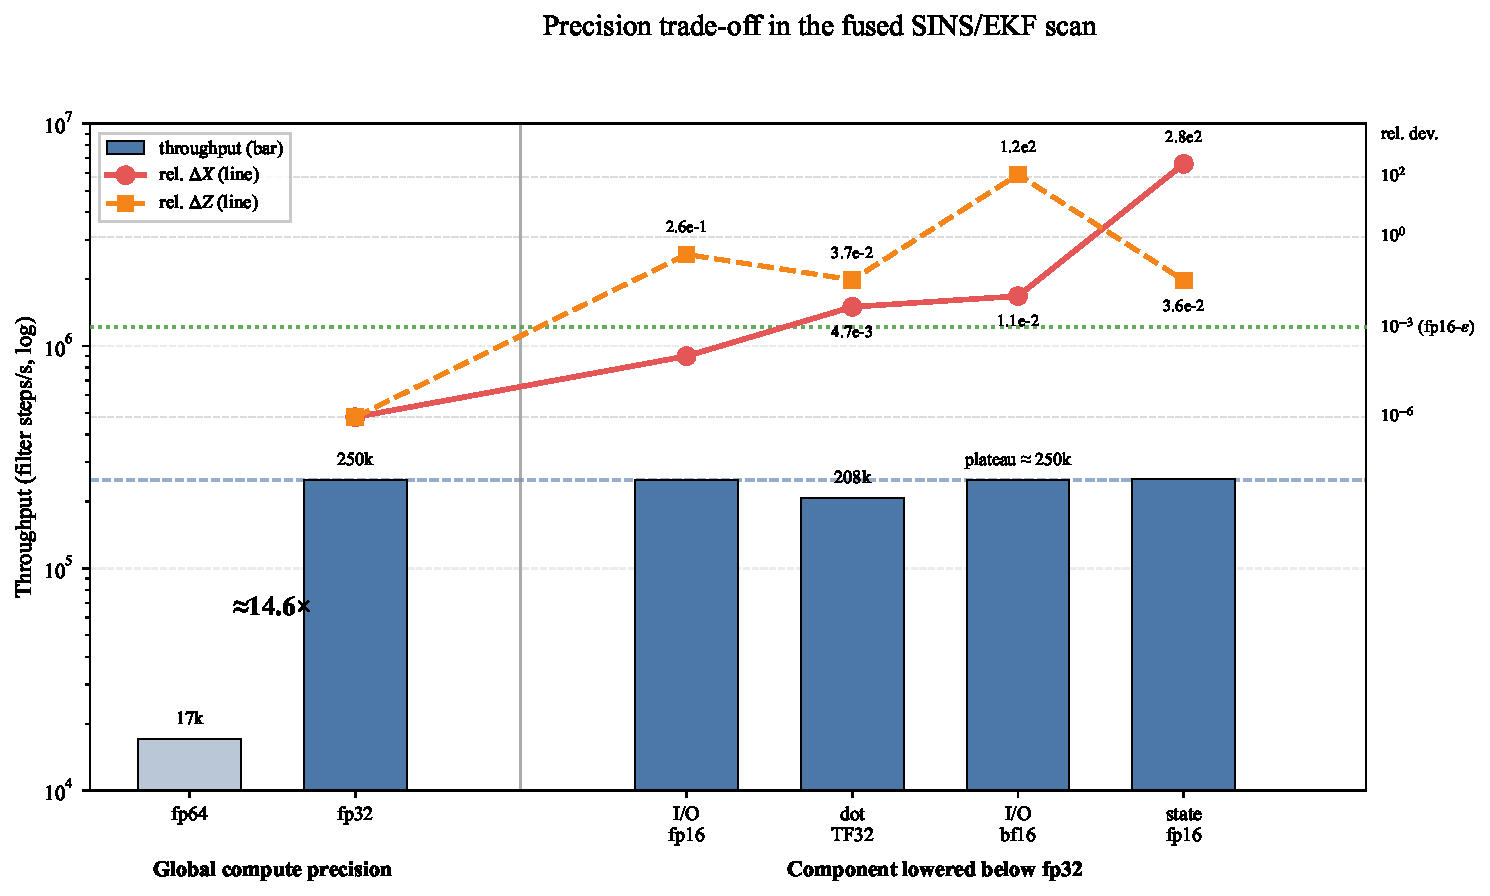
\includegraphics[width=\linewidth]{figures/3-motivation-precision_tradeoff.pdf}
  \caption{Precision trade-off in the fused SINS/EKF scan (\Cref{subsec:kernel-fusion}) over the full 166{,}667-step trajectory, measured on an H20. Bars (lower log axis) report end-to-end throughput, and lines (upper band, log axis) report the relative X/Z positioning deviation against the all-fp32 reference. The $10^{-3}$ line marks an fp16-$\varepsilon$ accuracy grade: bfloat16 sensor input and fp16 recurrent storage cross it and are unsafe for the long-horizon filter, whereas fp16 sensor input remains safely below it. TF32 matrix products sit near the boundary but add measurable deviation for negligible or negative throughput gain, and are consequently excluded by the component-aware plan.}
  \label{fig:precision-tradeoff}
\end{figure}

\subsection{Independent Trajectories Supply Device-Level Parallelism}
\label{subsec:motivation-trajectories}

The state and covariance at time $k$ depend on the result at time $k-1$, which limits temporal parallelism within one trajectory. Increasing the tile size or assigning more threads to an individual small matrix product cannot create work along this dependency chain. Kernel fusion removes dispatch and state-traffic overhead, but it does not change this limit: a single fused trajectory launches one 128-thread block, or four warps. On a Hopper-class H20, this block occupies only one SM at 6.25\% warp occupancy, leaving the device almost entirely idle, as summarized in \Cref{tab:motivation-utilization}. Reducing single-trajectory latency alone therefore cannot fill the GPU.

Simulation campaigns naturally provide an outer parallel dimension. Different noise realizations, obstacle configurations, and filter parameters produce independent trajectories with no shared recurrent state. Mapping these trajectories to separate blocks preserves the original update order within every filter while increasing aggregate device utilization. Scaling eventually becomes limited by the number of SMs and by register-constrained block residency. Together, the three observations above lead to whole-scan kernel fusion, component-aware precision, and multi-trajectory parallelism, which are developed in the next section.

\begin{table}[H]
  \centering
  \caption{Measured utilization for one fused fp32 trajectory on an H20. The kernel uses one 128-thread block per trajectory.}
  \label{tab:motivation-utilization}
  \begin{tabular}{@{}lr@{}}
    \toprule
    Characteristic & Value \\
    \midrule
    Grid / block size & $(1,1,1)$ / 128 threads (4 warps) \\
    SMs hosting the block & 1 of 78 \\
    Achieved occupancy & 6.25\% (4 / 64 warps) \\
    Device SM throughput & approximately 0.27\% \\
    \bottomrule
  \end{tabular}
\end{table}
